
%----------------------------------------------------------------------------------------
%	PREAMBUŁA
%----------------------------------------------------------------------------------------

\documentclass[12pt]{article}
\usepackage[polish]{babel}
\usepackage{polski}
\usepackage[utf8]{inputenc}
\usepackage{graphicx}
\usepackage{fancyhdr}
\usepackage{float}
\usepackage{graphicx}
\usepackage[hidelinks]{hyperref}
\usepackage{verbatim}
\usepackage{amsmath}
\usepackage{rotating}
\usepackage{listings}
\usepackage{xcolor}
\usepackage{subcaption}

\definecolor{lgray}{gray}{0.96}
\definecolor{lbcolor}{rgb}{0.9,0.9,0.9}
\lstset{
    framesep=2pt,
    breaklines=true,
    breakatwhitespace=true,
    basicstyle=\footnotesize,
    aboveskip={0.75\baselineskip},
    columns=flexible,
    showstringspaces=false,
    breaklines=true,
    prebreak = \raisebox{0ex}[0ex][0ex]{\ensuremath{\hookleftarrow}},
    frame=single,
    rulecolor=\color{lgray},
    showtabs=false,
    showspaces=false,
    showstringspaces=false,
    backgroundcolor=\color{lgray},
    identifierstyle=\ttfamily,
    keywordstyle=\color[rgb]{0,0,1},
    commentstyle=\color[rgb]{0.0,0.26,0.15},
    stringstyle=\color[rgb]{0.627,0.126,0.941}
}

\graphicspath{{static/}} 

\title{Sztuczne Sieci Neuronowe - Projekt}
\author{Aleksandra Poręba, Grzegorz Podsiadło}

\makeatletter
\let\thetitle\@title
\let\theauthor\@author
\let\thedate\@date
\makeatother

%----------------------------------------------------------------------------------------
%	STRONA TYTUŁOWA
%----------------------------------------------------------------------------------------
\begin{document}
\begin{center}
\textsc{\normalsize Wydział Fizyki i Informatyki Stosowanej}\\[2.0cm] 

\includegraphics[scale = 1]{logo.pdf}\\[1cm] 
\textsc{\Large Sztuczne Sieci Neuronowe}\\[0.4cm] 


{ \huge \bfseries \LARGE{Sprawozdanie z projektu} } 

\flushright \Large Aleksandra Poręba \\ Grzegorz Podsiadło

\vfill 

\center {\today}\\[2cm] 


\pagebreak 

\end{center}

%----------------------------------------------------------------------------------------
%	SPIS TREŚCI
%----------------------------------------------------------------------------------------
\setcounter{tocdepth}{2}
\tableofcontents
\pagebreak

%----------------------------------------------------------------------------------------
%	ZAWARTOŚĆ
%----------------------------------------------------------------------------------------

\pagestyle{fancy}
\fancyhf{}

\rhead{\theauthor}
\lhead{\thetitle}
\cfoot{\thepage}

\section{Wstęp}

\pagebreak
\section{Sieć neuronowa}
% że regresja, co testowaliśmy i dlaczego takie
% mlp 


\pagebreak
\section{Badanie wpływu ilości kolumn na wyniki sieci}
\subsection{Korelacja pomiędzy danymi}
W ramach projektu został obliczony współczynnik korelacji \textit{Pearsona} pomiędzy danymi z repozytorium. Dzięki niemu możemy sprawdzić jak bardzo zależne są od siebie dane, a dzięki temu dostosować informacje użyte do uczenia sieci.

Do obliczenia współczynnika korelacji została użyta funkcja pakietu MATLAB \verb\corr\.

\subsubsection {Korelacja pomiędzy wynikami egzaminów}
Na początku został wyznaczony współczynnik korelacji pomiędzy wynikami egzaminów. Otrzymane wyniki przedstawiono w tabeli poniżej.

\begin{table}[H]
\centering
\begin{tabular}{|c|c|c|} 
\hline
Egzamin 1 i 2 & Egzamin 1 i 3 & Egzamin 2 i 3  \\ 
\hline
0.6453 & 0.6435          &  0.8578 \\ 
\hline
\end{tabular}
\end{table}

Dla wszystkich kombinacji otrzymaliśmy wartości większe od $0.5$, możemy więc uznać, że dane są od siebie zależne. Największa korelacja występuje pomiędzy egzaminem 2 oraz 3 - współczynnik jest równy $0.86$.

Na rysunkach poniżej zależności pomiędzy zbiorami zostały przedstawione w sposób graficzny.

\begin{figure}[H]
\centering
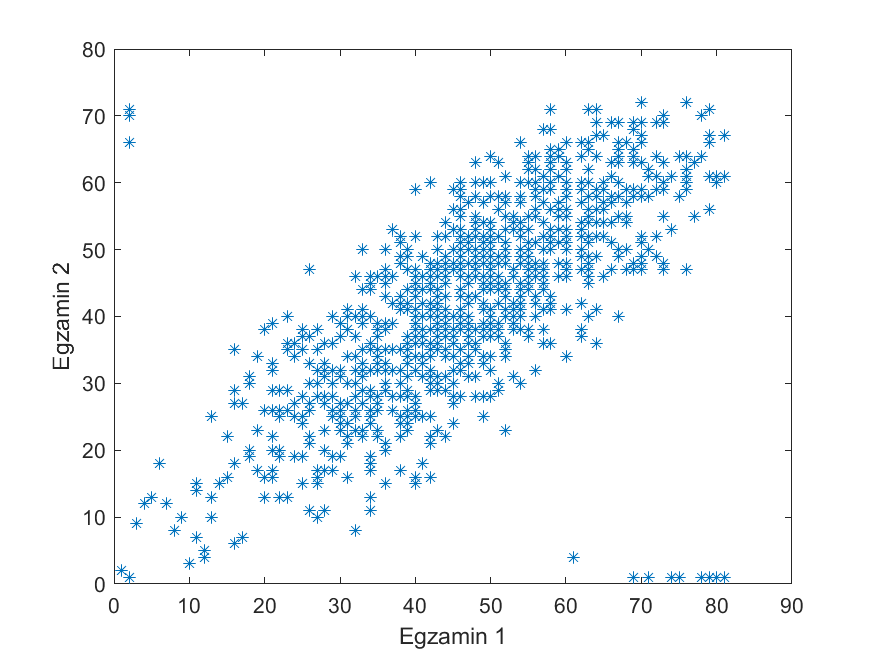
\includegraphics[width=0.45\textwidth]{korelacja_egzamin12.png}
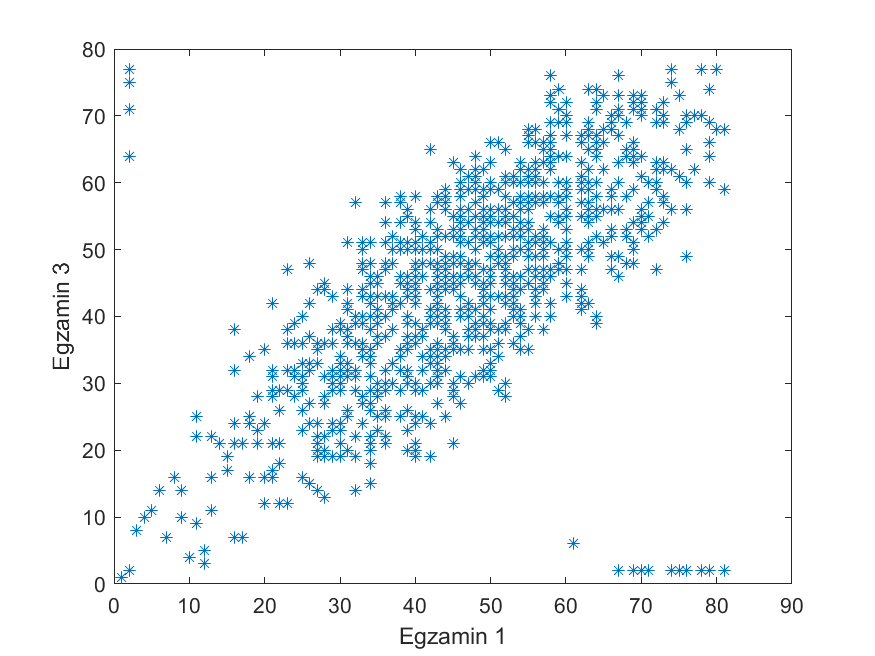
\includegraphics[width=0.45\textwidth]{korelacja_egzamin13.png}
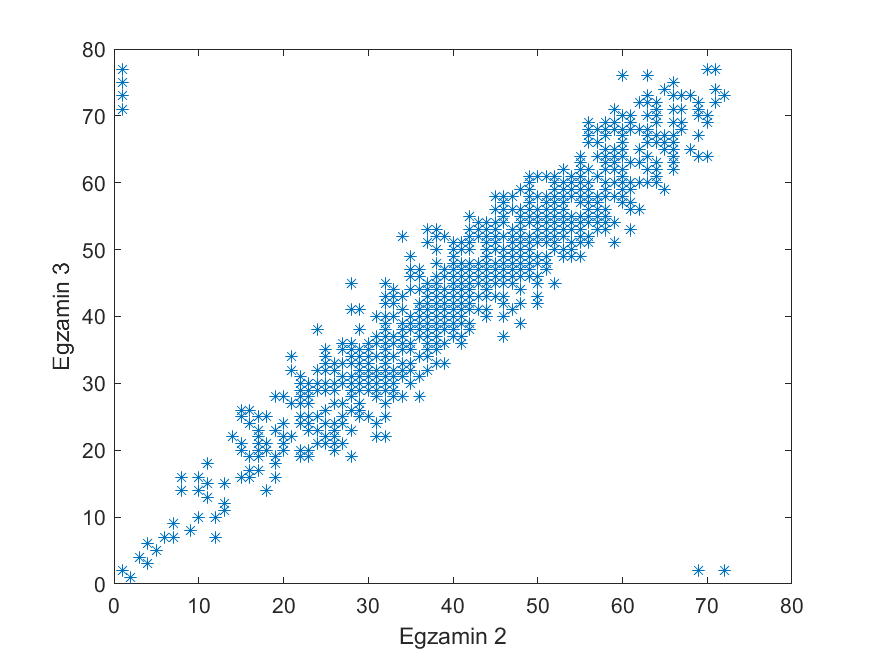
\includegraphics[width=0.45\textwidth]{korelacja_egzamin23.png}
\caption{Zależności pomiędzy wynikami egzaminów przedstawione w sposób graficzny.}
\end{figure}

\subsubsection {Korelacja pomiędzy czynnikami środowiskowymi a wynikami egzaminów}
W dalszej części analizy zbioru danych została zbadana zależność pomiędzy czynnikami, będącymi wejściem sieci neuronowej, a wynikami kolejnych egzaminów. Otrzymane współczynniki korelacji przedstawiono w tabeli poniżej.

\begin{table}[H]
\centering
\begin{tabular}{|c|c|c|c|} 
\hline
 Czynnik środowiskowy & Egzamin 1 & Egzamin 2 & Egzamin 3  \\ 
\hline
Płeć & 0.1558  &  -0.1886 &  -0.2396  \\ 
\hline
Rasa &  0.1771  &  0.0770   & 0.0907 \\ 
\hline
Wykształcenie rodzica &  -0.0584  & -0.0306 &  -0.0571  \\ 
\hline
Przystąpienie do kursu & 0.3269  &  0.1906  &  0.2182  \\ 
\hline
Dieta &  -0.1564  & -0.1838   & -0.2647  \\ 
\hline
\end{tabular}
\end{table}

Otrzymane wartości są dość niskie, nie istnieje wyraźna korelacja pomiędzy którąś z tych cech, a wynikami. Najmniejszą zależność obserwujemy pomiędzy wynikami, wykształceniem rodziców - są one najbliższe zeru. Największe znaczenie ma przystąpienie do kursu przygotowawczego, w dalszej kolejności dieta oraz płeć.

% nie dałam rysunków bo by ich było za dużo, można dodać potem jak uważasz że jakiś
% no np dla tych największych korelacji/najmniejszych

\subsection{Testowanie sieci neuronowej}
Dla wybranych najlepszych parametrów sieci zostało przeprowadzone uczenie z pomniejszoną ilością kolumn. Celem tego zabiegu było zbadanie, jaki wpływ mają te czynniki na poprawność działania sieci. %to jest nie po polsku xd

\pagebreak
\section{Przewidywanie wyniku egzaminu na podstawie pozostałych} %to też źle brzmi
Jak zostało zauważone podczas badania korelacji, wyniki egzaminów są od siebie zależne (wysoki współczynnik korelacji). Korzystając z wyników z dwóch egzaminów podjęto próbę stworzenia sieci obliczającą wynik z trzeciego egzaminu.

Otrzymane błędy testowania zostały przedstawione poniżej.

% rysunki z MSE oraz obok taki rysunek że jakie powinny być i jakie były przewidziane
% te tu nie są ostateczne, tylko chciałam zobaczyć jak to będize
\begin{figure}[H]
\centering
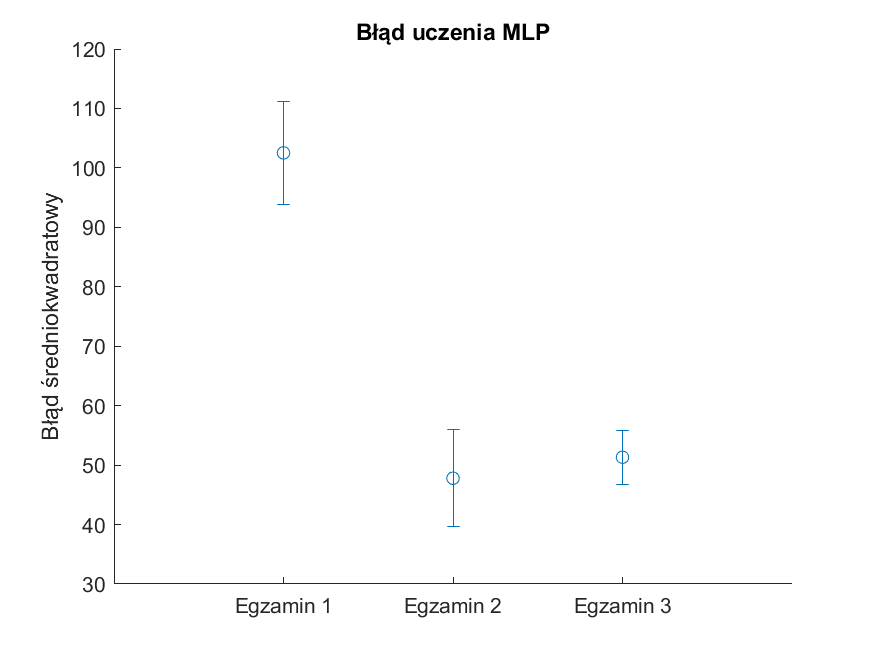
\includegraphics[width=0.45\textwidth]{cz3_egz_ucz.png}
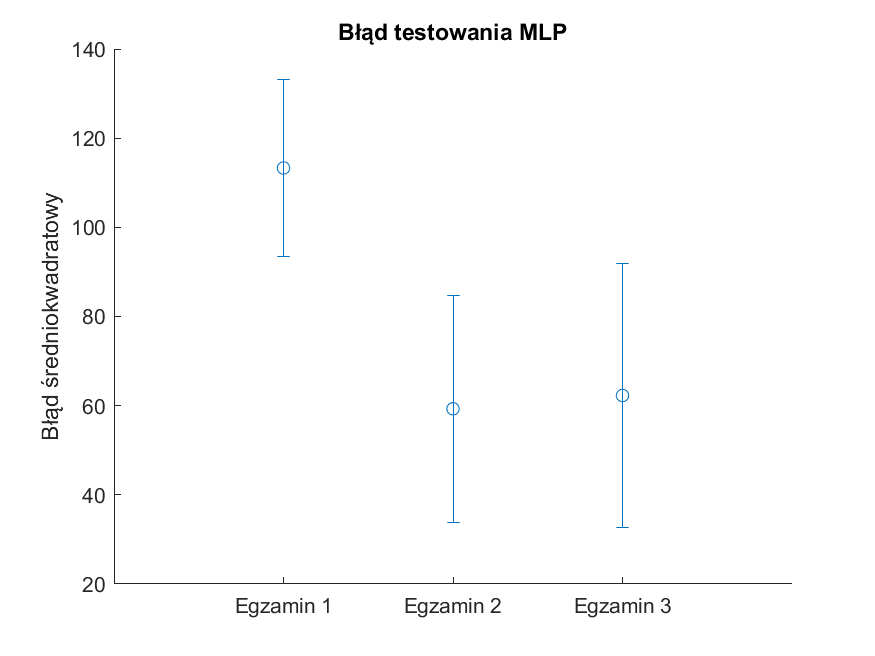
\includegraphics[width=0.45\textwidth]{cz3_egz_test.png}
\caption{Błąd uczenia i testowania sieci dla X prób dla kolejnych egzaminów}
\end{figure}

Na podstawie obserwacji wielkości błędów, można zauważyć, że dla egzaminów 2 oraz 3 sieć osiąga dobre wyniki - na poziomie wartości $50$.  Dla egzaminu 1 błędy przyjmują wartości dwa razy większe. 

Otrzymane wyniki można powiązać z analizowaną wcześniej korelacją danych - wyniki egzaminów 2 i 3 są ze sobą w większym stopniu powiązane, niż egzamin 1 z egzaminem 2 lub 3. 

% to że błędy są mniejsze niż na podstawie czynników środowiskowcyh

%  w sumie można ejszcze zrobić (jak zostanie czas) uczenie czynnikami + wynik pozostałych egzaminów, powinno być najlepiej

\pagebreak
\section{Podsumowanie}
% wnioski

\pagebreak

\begin{thebibliography}{9}


\end{thebibliography}

\end{document}